%==============================================================================
% DecisionGPT / R1 -- IEEE conference-format manuscript
%
% This manuscript reports the R1 controlled component-level evaluation. Every
% numerical value is carried verbatim from the frozen R1 artifacts:
%   experiments/r1/config.json
%   experiments/r1/statistical_results.json   (source results.json
%                                              SHA-256 9e302f1d1cf575940e62e9ab...)
%   experiments/r1/mechanism_results.json
%   experiments/r1/robustness_results.json
%   experiments/r1/independent_recheck.json   (75/75 checks reproduce)
%   experiments/r1/MACHINE_AUDIT.md           (26/26 checks pass)
% Pre-registration frozen at git commit 22ce18c965b6..., before the one-shot
% locked run. The R1 locked test was executed exactly once (4080 instances,
% 0 errors) and is NOT re-run, re-seeded, tuned, or modified here.
%
% Frozen prior artifacts, verified byte-identical before and after this write:
%   experiments/experiment_manifest.json  SHA-256 94aa419c703b1babb46597546...
%   experiments/paper_results_snapshot.json SHA-256 8e09d298ac3ba3cbdfe5cc7b...
%   docs/PAPER_DRAFT.md                    SHA-256 72e454490845788b0996fd0bb...
%   docs/ieee_paper/{main.tex,references.bib,README.md}  unchanged
% V1 = evaluation_complete; V2 = STOPPED_AT_PRELOCK_GATE (locked_test_run=false);
% R0/D0 unchanged; R3 NOT PROMOTED. No real SME data. No real LLM. No causal claim.
%
% Compile:  latexmk -pdf main.tex     (or: pdflatex; bibtex; pdflatex x2)
% Requires: IEEEtran.cls + IEEEtran.bst, graphicx, amsmath, amssymb, array,
%           booktabs, url, hyperref.
% Figures: figures/r1_figure{1..5}.pdf are provided (converted from the frozen
%   .svg via  python scripts/r1_figures_to_pdf.py ). The .svg originals are kept
%   alongside. \includegraphics uses no extension, so pdflatex picks the .pdf.
% NOTE: at the time this file was finalised no LaTeX toolchain (pdflatex/bibtex)
%   was available in the build environment, so the PDF was NOT compiled here;
%   only structural / numerical / citation validation was performed. Compile on
%   any TeX Live / MiKTeX / Overleaf install.
%==============================================================================
\documentclass[conference]{IEEEtran}
\IEEEoverridecommandlockouts

\usepackage[T1]{fontenc}
\usepackage{graphicx}
\usepackage{amsmath}
\usepackage{amssymb}
\usepackage{array}
\usepackage{booktabs}
\usepackage{url}
\usepackage[hidelinks]{hyperref}

\graphicspath{{figures/}}

\newcommand{\code}[1]{\texttt{#1}}
\newcommand{\dvb}{\ensuremath{D\!-\!B}}
\newcommand{\rb}{\ensuremath{r_{\mathrm{rb}}}}

\begin{document}

\title{Does a Multi-Agent Layer Help? A Controlled Component-Level Evaluation of
an Integrated Decision-Support Architecture for Data-Constrained SMEs}

%------------------------------------------------------------------------------
% AUTHOR BLOCK. Names, order, affiliation, corresponding-author email and the
% supervisor \thanks note are carried over verbatim from the project's frozen
% publication package (docs/ieee_paper/main.tex). No student registration
% numbers, ORCID iDs, funding, grants, or acknowledgements are asserted.
%------------------------------------------------------------------------------
\author{%
\IEEEauthorblockN{K. S. Sri Vardhan, R Rohit, K. Rahul, and Felix}
\IEEEauthorblockA{SCOPE, VIT-AP University, Vijayawada, Andhra Pradesh, India}
\thanks{Corresponding author: K. S. Sri Vardhan
(vardhan.23bce8389@vitapstudent.ac.in).}
\thanks{Supervisor: Prof.\ Yelepi Usha Rani, Professor, SCOPE, VIT-AP
University, Vijayawada, Andhra Pradesh, India (usharani.y@vitap.ac.in).}
}

\maketitle

%==============================================================================
\begin{abstract}
We report a pre-registered, controlled, synthetic-scenario evaluation that asks
which components of a goal-to-strategy decision-support pipeline carry
measurable value, and in particular whether a rule-based multi-agent evaluation
and risk-aware optimisation stack improves decision quality over a functioning
business decision-simulation layer. The study evaluates a \emph{research-only}
corrected version of the pipeline: we first show, by feature-attribution and a
direct price sweep, that the shipped decision-simulation layer is insensitive to
the decision variables it is meant to reason about, and we replace only its
scenario-side demand and revenue projection with a minimal constant-elasticity
model whose coefficients are estimated from each business's own history. All
other components---baseline forecast, risk score, candidate action set, three
evaluation agents, optimiser, and control flow---are unchanged and operate on
the corrected projections. Against an exogenous additive-linear objective of a
different functional form, evaluated on 12 pre-registered locked scenario
families ($12\times34 = 408$ structural scenarios, 10 seeds each, 4080 decisions
per condition, 0 errors), the corrected decision-simulation layer (condition~B)
significantly reduces normalised regret relative to a prediction-only pipeline
(condition~A):
mean difference $-0.044$, 95\% cluster-bootstrap CI $[-0.084,-0.002]$,
Holm-adjusted $p=1\times10^{-8}$. Adding a single evaluation agent (condition~C)
changes regret by a non-significant $-0.054$ (Holm $p=0.61$). The full
downstream stack (condition~D) \emph{increases} regret relative to B: mean
difference $+0.085$, 95\% CI $[+0.048,+0.123]$, Wilcoxon $p=5.4\times10^{-10}$,
Holm $p\approx0$, matched-pairs rank-biserial $-0.469$; D is worse than B on
274 of 408 scenarios and better on 99. The direction is preserved under
leave-one-family-out (range $+0.050$ to $+0.159$) and under all 18
pre-registered robustness perturbations. A trace analysis localises---but does
not causally prove---the degradation to the transition from C to D
(mean $+0.139$, Holm $p\approx0$): D overrides B's action on 57\% of decisions
and, when it does, worsens the outcome about twice as often as it improves it
($1573$ vs $763$), and D's optimal-action rate falls from B's 62.5\% to 34.6\%.
DecisionGPT's own internal goal-achievement metric shows the same ordering
($B=0.496$, $D=0.364$). The result is \textbf{negative} for the tested
deterministic multi-agent configuration in this environment. We make no claim of
real-world, SME, causal, ROI, or deployment effect; no real large-language-model
agents were evaluated; and a negative result here does not show that multi-agent
architectures are unhelpful in general. The contribution is the diagnosis, the
minimal-correction methodology, a mechanism-characterised negative result, and a
fully reproducible analysis package in which every headline statistic is
independently recomputed from the raw results (75/75).
\end{abstract}

\begin{IEEEkeywords}
decision-support systems, prescriptive analytics, controlled evaluation,
component ablation, multi-agent systems, negative results, price elasticity,
risk-aware optimization, reproducibility, pre-registration
\end{IEEEkeywords}

%==============================================================================
\section{Introduction}
Integrated decision-support architectures increasingly stack a predictive model,
a scenario or ``digital'' simulation layer, one or more evaluation agents, a
risk model, and an optimiser, on the assumption that each added layer refines
the recommendation of the last~\cite{Lepenioti2020,Arnott2014}. This assumption
is rarely tested at the component level. When a stacked system is evaluated end
to end and performs well, it is unclear which layer earned the result; when it
performs poorly, it is unclear which layer to fix. Recent work on multi-agent
LLM systems documents that added agents can introduce coordination and
error-propagation failures rather than remove
them~\cite{Wang2024,Smit2024,Huang2024,Cemri2025}, which makes a controlled,
per-component measurement worthwhile even---especially---when the result is
negative.

This paper performs such a measurement for one concrete architecture, aimed at
data-constrained small and medium enterprises (SMEs)~\cite{OECD2021,Buteau2021}.
Our position is that adding reasoning or optimisation layers does not by itself
guarantee better decisions, so components should be measured independently rather
than assumed to compound. The research questions (formalised in
Section~\ref{sec:rq}) are: whether a responsive decision-simulation layer
improves on prediction alone (RQ1); whether the tested downstream
agent/risk/optimisation stack improves on that decision-simulation layer (RQ2,
scoped to \emph{this} deterministic configuration, not multi-agent systems in
general); and under which controlled scenario mechanisms that stack helps or
hurts (RQ3).

A prerequisite forced a design decision. Feature attribution and a direct price
sweep (Section~\ref{sec:diag}) show that the pipeline's shipped
decision-simulation layer is essentially insensitive to the price and marketing
decisions it is supposed to evaluate: its projected units are flat across a
threefold price change. Evaluating the downstream stack on top of a
non-responsive simulation layer would answer a different, less interesting
question. We therefore define a \emph{research-only} variant, R1, that replaces
\emph{only} the scenario-side demand/revenue/profit projection with a minimal
constant-elasticity model estimated from each business's own transaction history
(Section~\ref{sec:correction}), and leave every other component byte-identical.
R1 is never presented as the production system, and the paper's central contrast
(D vs B) is between two conditions that both inherit this correction, so its sign
does not depend on the exact elasticity form.

Our findings, on a pre-registered synthetic benchmark: the corrected
decision-simulation layer is the only component that measurably lowers regret
(B beats A); a single evaluation agent is inert (C $\approx$ B); and the full
stack \emph{raises} regret (D worse than B and than C), robustly and with a
diagnosable mechanism. We state plainly what this does and does not establish
(Section~\ref{sec:threats}).

%==============================================================================
\section{Related Work}
\textbf{Prescriptive and decision-support analytics.} Surveys of prescriptive
analytics and of decision-support systems describe the predict-then-optimise and
simulate-then-decide patterns our system instantiates~\cite{Lepenioti2020,Arnott2014}.
Predictive modelling practice for explanation vs prediction is
treated by Shmueli~\cite{Shmueli2011}.

\textbf{Digital twins vs digital models.} Our scenario layer is, in the
terminology of Kritzinger et al.~\cite{Kritzinger2018}, a digital \emph{model}:
a manually exercised simulation with no automated state feedback from the
business. We use ``decision-simulation layer'' throughout and avoid ``digital
twin''~\cite{Grieves2017,Tao2019,Jones2020}.

\textbf{Multi-agent systems and their failure modes.} LLM- and rule-based
multi-agent pipelines are widely proposed for analytical
tasks~\cite{Du2023,Liang2024,Li2024,Zheng2023}. A parallel line of work
catalogues where added agents hurt: inter-agent error amplification and
coordination failure~\cite{Wang2024}, debate that does not converge to
truth~\cite{Smit2024,Huang2024}, and a taxonomy of multi-agent failure
modes~\cite{Cemri2025,Yang2024}. Our negative result is consistent with this
line but is obtained by a component ablation rather than an end-to-end contest.

\textbf{Risk-aware optimisation.} The degradation we localise involves a
risk-penalty term in the optimiser~\cite{Garcia2015}. We treat the mechanism
analysis as associational.

\textbf{Evaluation methodology.} We follow pre-registration and
reproducibility guidance~\cite{Nosek2018,Baker2016,Pineau2021}, use the Wilcoxon
signed-rank test~\cite{Wilcoxon1945} with matched-pairs rank-biserial effect
size~\cite{Kerby2014,Fritz2012}, Holm-type control of the confirmatory
family~\cite{Benjamini1995}. Following~\cite{Hyndman2006}, we never label a
regret metric or error metric as ``accuracy'' (the endpoint is normalised
regret throughout). We report an effect-direction result and its
interval rather than leaning on a single threshold~\cite{Wasserstein2016,Rosenthal1979}.

%==============================================================================
\section{Scope and Non-Goals}\label{sec:scope}
This is a controlled synthetic evaluation. It \emph{does} establish, within the
tested environment: the relative ordering of pipeline components on an exogenous
objective; the sign, interval and robustness of the D-vs-B contrast; and an
associational localisation of the degradation.

It \emph{does not} establish, and the paper never claims: real-world or SME
decision outcomes; causal business impact, ROI, or customer effects;
effectiveness or superiority of DecisionGPT as a product; any statement about
large-language-model agents (none were evaluated---the three agents are
deterministic rule-based components); or a general claim that multi-agent
architectures help or hurt. No real SME data were used at any point. R1 is a
research-only variant; the production configuration is unchanged
(\code{R0}/\code{D0}).

%==============================================================================
\section{Research Questions}\label{sec:rq}
\begin{description}
  \item[RQ1.] Does the decision-simulation layer improve decision quality beyond
        prediction alone? (Contrast $B\text{\_vs\_}A$.)
  \item[RQ2.] Does the downstream agent/risk/optimisation stack improve decision
        quality beyond the decision-simulation layer? (Contrast $D\text{\_vs\_}B$,
        with $C\text{\_vs\_}B$ and $D\text{\_vs\_}C$ isolating the single-agent
        and the risk/optimiser steps.) RQ2 concerns the \emph{tested
        deterministic configuration}; it is not a claim about multi-agent systems
        in general.
  \item[RQ3.] Under which controlled scenario mechanisms does the downstream
        stack help or hurt? (Per-family effects, leave-one-family-out, and the
        associational mechanism analysis.)
\end{description}

%==============================================================================
\section{System Under Test}\label{sec:sut}
The pipeline maps a natural-language business goal to a recommended strategy
(a bounded change to price and marketing spend) through: (i)~a baseline demand
forecast; (ii)~a candidate action set; (iii)~a decision-simulation layer that
projects units, revenue and profit for each candidate; (iv)~a risk score;
(v)~three rule-based evaluation agents (a forecasting critic, a risk critic, and
a constraint/feasibility critic); and (vi)~a risk-aware optimiser that scores
candidates with a value term minus a risk-penalty term and returns the argmax.

Figure~\ref{fig:arch} shows the architecture and information boundary. We
evaluate four nested conditions:
\begin{itemize}
  \item \textbf{A --- prediction only.} The recommendation is the
        smallest-magnitude candidate action (the pipeline's behaviour when no
        simulation/agent/optimiser signal is available); scored via the
        ground-truth no-op action.
  \item \textbf{B --- + decision simulation.} A is extended with the R1-corrected
        decision-simulation layer; the recommendation is its regret-minimising
        candidate (argmax of projected objective).
  \item \textbf{C --- + one agent.} B is extended with a single evaluation
        agent.
  \item \textbf{D --- full system.} All three agents plus the risk-aware
        optimiser, i.e.\ \code{decision\_service.analyze\_goal} with default
        options (\code{R0}/\code{D0}).
\end{itemize}
A $\subset$ B $\subset$ C $\subset$ D by construction; each contrast isolates one
added component.

\begin{figure}[!t]
\centering
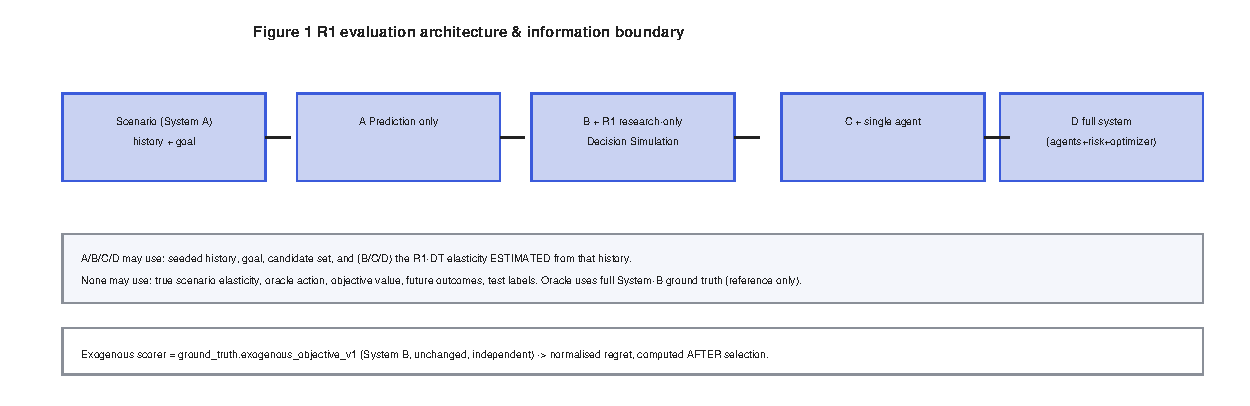
\includegraphics[width=\columnwidth]{r1_figure1}
\caption{R1 architecture and information boundary. Conditions A$\subset$B$\subset$C$\subset$D;
System~A (log-linear history) and System~B (additive-linear exogenous objective)
are distinct functional forms coupled only by a noisy monotone parameter map;
the research-only correction replaces only the scenario-side units/revenue/profit
projection.}
\label{fig:arch}
\end{figure}

%==============================================================================
\section{The Decision-Simulation Bottleneck: Diagnosis}\label{sec:diag}
Three independent observations show the shipped decision-simulation layer does
not respond to the decision variables (full detail in the frozen diagnostic
report):
\begin{enumerate}
  \item \textbf{Feature attribution.} In the production demand forecaster, the
        summed SHAP importance of \code{price} and \code{marketing\_spend} is
        about $2.2\%$ of the total, while the autoregressive level (lag and
        rolling-mean features) carries about $77\%$.
  \item \textbf{Direct sweep.} Sweeping price threefold ($50\to150$) with all
        else fixed changes the model's predicted units by a range of exactly
        $0.0$ (flat).
  \item \textbf{Revenue monotonicity.} The simulation then computes
        \code{expected\_revenue} $=$ \code{units} $\times$ \code{price} on the
        flat units, so projected revenue is monotone increasing in price and the
        layer's argmax is the maximum candidate price increase ($+10\%$) in
        essentially every scenario, i.e.\ a degenerate policy (2 distinct
        actions across 272 development executions).
\end{enumerate}
The forecaster's training series has a \code{price} mean near $1{,}430$ against
evaluation prices spanning roughly $80$--$3{,}000$, and a \emph{wrong-signed}
(weakly positive) crude price/units slope; the degeneracy is thus a property of
the shipped model and its inputs, not of the evaluation environment.

%==============================================================================
\section{Research-Only Correction (R1)}\label{sec:correction}
R1 replaces only the scenario-side \code{expected\_units\_sold},
\code{expected\_revenue} and \code{expected\_profit}. For a candidate that
changes price by $\Delta p\%$ and marketing spend by $\Delta m\%$:
\begin{equation}
u = u_{\mathrm{base}}\cdot
\mathrm{clip}\!\big((1+\Delta p/100)^{\hat\varepsilon},0,5\big)\cdot
\mathrm{clip}\!\big((1+\Delta m/100)^{\hat a},0,5\big)\cdot f_{\mathrm{cap}},
\end{equation}
where $u_{\mathrm{base}}$ is the unchanged baseline forecast level,
$f_{\mathrm{cap}}$ applies the known inventory/capacity ceiling, and
$\hat\varepsilon\in[-4,-0.05]$, $\hat a\in[0,1]$ are estimated by ordinary least
squares of $\log(\text{units})$ on $\log(\text{price})$,
$\log(\text{marketing\_spend})$ and weekday dummies over the business's own
seeded transaction history. Revenue and profit are recomputed from $u$ using the
baseline-implied unit price and unit cost. The clip on $\hat\varepsilon$ only
enforces a downward-sloping demand curve---an economic prior, not a tuned
value---and no coefficient is hand-set. The estimator falls back to the scenario
generator's nominal elasticity when the history is unusable (fewer than 20 rows,
near-zero log-price variance, or rank deficiency); on the locked run the
\textbf{fallback rate was $0.0\%$}. On the development/validation partition the
median absolute error of $\hat\varepsilon$ was $0.084$.

The baseline forecast level, the risk score, the candidate set, the three
agents, the optimiser and the control flow are unchanged and run on the
corrected projections. The correction is installed per instance by the R1
harness and removed afterwards; the production simulation file is byte-identical
on disk.

%==============================================================================
\section{Information Boundary}\label{sec:info}
All four conditions receive the same seeded history, goal and candidate set.
B, C and D additionally receive $\hat\varepsilon,\hat a$ \emph{estimated from
that same history}. No condition receives the true scenario elasticity, the
oracle action, the objective value, future outcomes, or test-set labels. The R1
correction module imports no ground-truth, oracle, or objective code (verified by
static import analysis); the exogenous objective is evaluated strictly after
action selection; and the oracle is reproduced by independent enumeration on all
408 locked scenarios.

%==============================================================================
\section{Synthetic Environment and Scenario Families}\label{sec:env}
The history-generating environment (``System~A'') is a log-linear power-law
model in which demand responds to historical price and marketing. Scenarios are
drawn from \textbf{27 families}; a stratified round-robin rule assigns
\textbf{12 families to the locked test set}
(\code{asymmetric\_risk}, \code{capacity\_bound}, \code{delayed\_price},
\code{demand\_saturation}, \code{noisy\_observations}, \code{nonlinear\_response},
\code{price\_elastic}, \code{promotion\_threshold}, \code{regime\_shift},
\code{strong\_seasonality}, \code{weak\_marketing}, \code{weak\_seasonality}),
11 families to the development partition and 4 to the validation partition. The
locked set is
\textbf{34 structural scenarios per family $\times$ 12 $=$ 408 scenarios},
each run with \textbf{10 seeds} ($4080$ decisions per condition). The master
seed ($20260907$), all family parameters, the partition assignment, and the
suite checksum (\code{cd73f0d5\ldots}) were frozen in the pre-registration.
Table~\ref{tab:families} lists the 12 locked families and the decision mechanism
each isolates.

\begin{table}[!t]
\caption{The 12 pre-registered locked scenario families and the decision
mechanism each stresses. Each family contributes 34 structural scenarios
$\times$ 10 seeds $=$ 340 decisions per condition.}
\label{tab:families}
\centering
\begin{tabular}{ll}
\toprule
Family & Mechanism stressed \\
\midrule
\code{price\_elastic}       & strong price response; cutting price is optimal \\
\code{weak\_marketing}      & marketing lever near-inert \\
\code{strong\_seasonality}  & large periodic demand component \\
\code{weak\_seasonality}    & small periodic component; easy to over-fit \\
\code{capacity\_bound}      & binding supply/inventory ceiling \\
\code{delayed\_price}       & lagged price effect on demand \\
\code{asymmetric\_risk}     & downside-skewed outcome distribution \\
\code{noisy\_observations}  & high observation noise in history \\
\code{regime\_shift}        & structural break partway through history \\
\code{promotion\_threshold} & step change once a discount threshold is crossed \\
\code{nonlinear\_response}  & censored / saturating demand curve \\
\code{demand\_saturation}   & demand plateaus at high volume (censored) \\
\bottomrule
\end{tabular}
\end{table}

%==============================================================================
\section{Ground-Truth Objective and Regret}\label{sec:gt}
The scoring objective (``System~B'') is an \emph{additive-linear} function of the
realised decision---a different functional form from both the log-linear history
engine and the constant-elasticity correction. Its module imports only the
standard library plus \code{numpy}/\code{scipy} (statically verified) and is
byte-identical to the version used in the project's earlier evaluations. The
coupling between the history family parameters and the objective parameters is a
noisy monotone map (e.g.\ elasticity
$=\mathrm{clip}(a_{\mathrm{elast}}+\mathcal{N}(0,0.35),\,-3.0,\,-0.15)$), not
shared code.

For each scenario the \textbf{normalised regret} of an action is
$(\,v^\star - v_{\mathrm{action}}\,)/(\,v^\star - v_{\mathrm{worst}}\,)$, where
$v^\star$ is the oracle (enumeration) optimum and $v_{\mathrm{worst}}$ the worst
feasible action: $0$ is optimal, $1$ is worst feasible, lower is better. The
unit of analysis is the scenario; the 10 seeds are averaged to the scenario mean
before any test.

%==============================================================================
\section{Baselines}\label{sec:baselines}
Alongside A/B/C/D we report four reference policies: \textbf{naive} (a fixed
do-something rule), \textbf{greedy} (one-step objective-greedy),
\textbf{classical optimiser} (a bounded numerical optimiser with analytic access
to the objective), and the \textbf{oracle} (enumeration optimum). The greedy,
classical and oracle references have privileged access to the objective and are
labelled \emph{external computational benchmarks}, not architecture competitors;
the paper's claims rest on the A/B/C/D contrasts, which share information and the
action space.

%==============================================================================
\section{Experimental Design and Pre-Registration}\label{sec:design}
The pre-registration (frozen at git \code{22ce18c}, before the run) fixes: the
27 families and their parameters; the partition rule and resulting locked
families; $N$ and the 10 seeds; the four conditions; the exogenous regret
endpoint; the confirmatory contrast family
$\{B\text{\_vs\_}A,\ C\text{\_vs\_}B,\ D\text{\_vs\_}C,\ D\text{\_vs\_}B\}$;
the primary contrast $D\text{\_vs\_}B$; a minimum effect of interest
$\mathrm{MEI}=0.05$; $\alpha=0.05$; the analysis code; and the four-way
classification \{SUPPORTED, PROMISING, NULL-INCONCLUSIVE, NEGATIVE\}. A pre-lock
gate (12/12 GO) confirmed, on development/validation only, that the corrected
layer is responsive (responsive fraction $0.917$; 6 distinct actions selected;
correlation between family elasticity and B's price move $+0.40$) before the
pre-registration was frozen. The locked test was then run \textbf{once}; there
was no re-run, no tuning, and no post-hoc exclusion (0 rows excluded).

%==============================================================================
\section{Statistical Analysis Plan}\label{sec:stats}
Per contrast $X\text{\_vs\_}Y$ we report the mean and median of
$(\,\mathrm{regret}_X-\mathrm{regret}_Y\,)$ over the 408 scenario means
(negative $=$ $X$ better); a paired \textbf{scenario cluster bootstrap} 95\%
percentile interval (10\,000 resamples, seed $12345$); the paired
\textbf{Wilcoxon signed-rank} $p$; the \textbf{matched-pairs rank-biserial}
effect size \rb; and wins/ties/losses. The four confirmatory contrasts are
corrected together by the Holm step-down procedure; raw and adjusted $p$ are
both reported. Secondary contrasts (D vs A, naive, greedy, classical, oracle;
A/B/C vs oracle) are descriptive and excluded from the correction.
$D\text{\_vs\_}B$ is classified \textbf{NEGATIVE} iff
$\mathrm{mean}(\dvb)>0$, the bootstrap CI excludes $0$, $|\mathrm{mean}|>\mathrm{MEI}$,
Holm $p<0.05$, the sign survives leave-one-family-out, and the mechanism is
plausible.

%==============================================================================
\section{Power}\label{sec:power}
A simulation-based power calculation used \emph{development-stage variance only}
(pilot $D\text{\_vs\_}B$ standard deviation $0.282$, rounded up to $0.30$) and
was computed \emph{before} the locked run: at $\mathrm{MEI}=0.05$, $N=408$,
10 seeds, the estimated power was \textbf{0.894}. $N$ had been raised from a
126-scenario sizing draft (power $\approx0.40$) by making the partition
locked-heavy; the effect of interest was not lowered. The power routine does not
model exact ties; the locked contrast has $35/408$ ties ($n_{\neq}=373$), so
achieved power is modestly below $0.894$. The observed effect ($0.085$) is
$1.7\times$ the MEI and the $p$-value is $5.4\times10^{-10}$, so this does not
affect the conclusion.

%==============================================================================
\section{Results: Component Ladder}\label{sec:ladder}
Table~\ref{tab:ladder} gives mean regret, mean normalised performance, and the
pipeline's internal secondary goal-achievement metric for every policy.
Figure~\ref{fig:ladder} plots the regret ladder. The ordering is
oracle $<$ classical optimiser $<$ C $<$ greedy $<$ B $<$ A $<$ D $<$ naive.
Two facts stand out: (i)~B and C both beat A, so value enters at the
decision-simulation layer; (ii)~D has \emph{higher} regret than A, B and C, and
is beaten by the greedy one-step reference.

\begin{table}[!t]
\caption{Component and baseline ladder on the 408 locked scenarios
(10 seeds each). Regret: $0$ optimal, lower better. ``Perf.'' is
$1-$regret-like normalised performance. ``Goal ach.'' is the pipeline's internal
secondary metric (higher better; undefined for A).}
\label{tab:ladder}
\centering
\begin{tabular}{lccc}
\toprule
Policy & Mean regret & Perf. & Goal ach. \\
\midrule
Oracle (enumeration)      & 0.000 & 1.000 & --- \\
Classical optimiser$^\dagger$ & 0.089 & --- & --- \\
C (+ one agent)           & 0.162 & 0.838 & 0.454 \\
Greedy$^\dagger$          & 0.197 & --- & --- \\
B (+ decision simulation) & 0.216 & 0.784 & 0.496 \\
A (prediction only)       & 0.259 & 0.741 & --- \\
D (full system)           & 0.301 & 0.699 & 0.364 \\
Naive                     & 0.367 & --- & --- \\
\bottomrule
\end{tabular}\\[2pt]
{\footnotesize $^\dagger$ Has analytic access to the objective; external
computational benchmark, not an architecture competitor.}
\end{table}

\begin{figure}[!t]
\centering
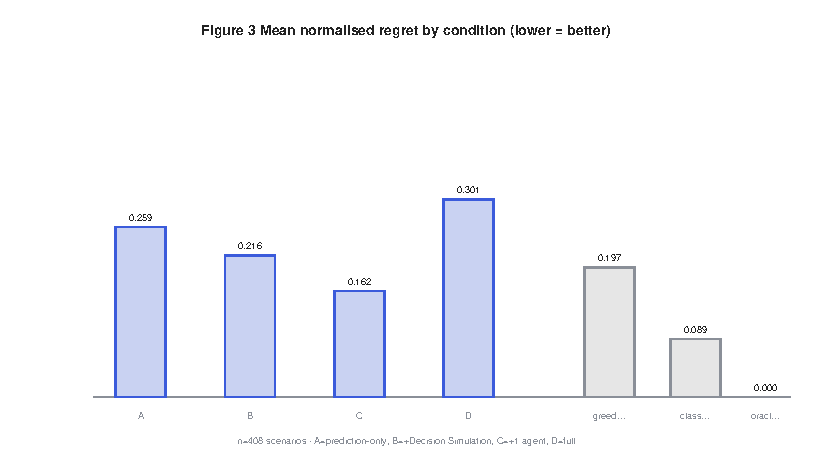
\includegraphics[width=\columnwidth]{r1_figure3}
\caption{Mean-regret ladder (lower is better): oracle $0.000$, classical
optimiser $0.089$, C $0.162$, greedy $0.197$, B $0.216$, A $0.259$, D $0.301$,
naive $0.367$. Value enters at B; D is below A, B and C.}
\label{fig:ladder}
\end{figure}

%==============================================================================
\section{Results: Confirmatory Contrasts}\label{sec:confirm}
Table~\ref{tab:confirm} reports the four pre-registered contrasts.
Figure~\ref{fig:paired} shows the sorted per-scenario $\dvb$ differences.

\begin{itemize}
  \item \textbf{RQ1 --- $B\text{\_vs\_}A$: B better.} Mean $-0.044$, 95\% CI
        $[-0.084,-0.002]$, Wilcoxon $p=4.8\times10^{-9}$, Holm
        $p=1\times10^{-8}$, \rb${}=+0.43$; B better on 292 of 408 scenarios,
        worse on 116. A functioning decision-simulation layer improves on
        prediction alone.
  \item \textbf{RQ2, step 1 --- $C\text{\_vs\_}B$: null.} Mean $-0.054$, 95\% CI
        $[-0.088,-0.020]$, Wilcoxon $p=0.61$, Holm $p=0.61$ (not rejected),
        \rb${}=-0.08$; 100 exact ties. The single agent adds no
        statistically supported incremental value.
  \item \textbf{RQ2, step 2 --- $D\text{\_vs\_}C$: D worse.} Mean $+0.139$,
        95\% CI $[+0.116,+0.162]$, Wilcoxon $p=1.7\times10^{-31}$, Holm
        $p\approx0$, \rb${}=-0.63$; D worse on 280 of 408. The degradation
        appears at the transition to the full risk/optimiser stack.
  \item \textbf{RQ2, primary --- $D\text{\_vs\_}B$: D worse.} Mean $+0.085$,
        95\% CI $[+0.048,+0.123]$, Wilcoxon $p=5.4\times10^{-10}$, Holm
        $p\approx0$, \rb${}=-0.469$; D better on 99, tie on 35, D worse on 274
        of 408 ($n_{\neq}=373$). Sign convention: positive $\dvb$ means D has the
        \emph{higher} regret, i.e.\ D is worse. Pre-registered classification:
        \textbf{NEGATIVE}.
\end{itemize}

Secondary contrasts (Table~\ref{tab:secondary}) are consistent: D vs A is a
non-significant $+0.042$ (Wilcoxon $p=0.13$; bootstrap CI $[+0.016,+0.068]$),
so D is at best no better than prediction alone; D beats only the naive
reference ($-0.066$, $p=8.1\times10^{-7}$) and loses to greedy ($+0.104$),
the classical optimiser ($+0.212$) and the oracle ($+0.301$).

\begin{table*}[!t]
\caption{Pre-registered confirmatory contrasts on 408 scenario means.
$\Delta = \mathrm{regret}_{\text{first}}-\mathrm{regret}_{\text{second}}$;
negative $=$ first better. CI is the paired scenario cluster bootstrap
(10\,000 resamples, seed 12345, percentile). Holm over the four-contrast family.
W/T/L counts first-better / tie / first-worse.}
\label{tab:confirm}
\centering
\begin{tabular}{lccccccc}
\toprule
Contrast & Mean $\Delta$ & Median $\Delta$ & 95\% CI & Wilcoxon $p$ & Holm $p$ & \rb & W/T/L \\
\midrule
$B\text{\_vs\_}A$ & $-0.0436$ & $-0.1936$ & $[-0.0843,\,-0.0021]$ & $4.8\times10^{-9}$ & $1\times10^{-8}$ & $+0.431$ & $292/0/116$ \\
$C\text{\_vs\_}B$ & $-0.0540$ & $0.0000$ & $[-0.0881,\,-0.0204]$ & $0.609$ & $0.609$ & $-0.084$ & $141/100/167$ \\
$D\text{\_vs\_}C$ & $+0.1392$ & $+0.0558$ & $[+0.1158,\,+0.1623]$ & $1.7\times10^{-31}$ & $\approx0$ & $-0.633$ & $63/65/280$ \\
$D\text{\_vs\_}B$ (primary) & $+0.0852$ & $+0.1000$ & $[+0.0479,\,+0.1231]$ & $5.4\times10^{-10}$ & $\approx0$ & $-0.469$ & $99/35/274$ \\
\bottomrule
\end{tabular}
\end{table*}

\begin{table}[!t]
\caption{Secondary contrasts for D (descriptive; not Holm-corrected).
$\Delta = \mathrm{regret}_D-\mathrm{regret}_{\text{ref}}$; negative $=$ D better.}
\label{tab:secondary}
\centering
\begin{tabular}{lcccc}
\toprule
Reference & Mean $\Delta$ & 95\% CI & Wilcoxon $p$ & W/T/L \\
\midrule
A                   & $+0.0417$ & $[+0.016,+0.068]$ & $0.13$              & $198/1/209$ \\
naive               & $-0.0662$ & $[-0.095,-0.037]$ & $8.1\times10^{-7}$  & $252/0/156$ \\
greedy$^\dagger$    & $+0.1036$ & $[+0.079,+0.129]$ & $7.9\times10^{-11}$ & $140/0/268$ \\
classical opt.$^\dagger$ & $+0.2123$ & $[+0.183,+0.241]$ & $1.0\times10^{-33}$ & $66/22/320$ \\
oracle$^\dagger$    & $+0.3008$ & $[+0.278,+0.324]$ & $1.6\times10^{-63}$ & $0/31/377$ \\
\bottomrule
\end{tabular}\\[2pt]
{\footnotesize $^\dagger$ Analytic access to the objective.}
\end{table}

\begin{figure}[!t]
\centering
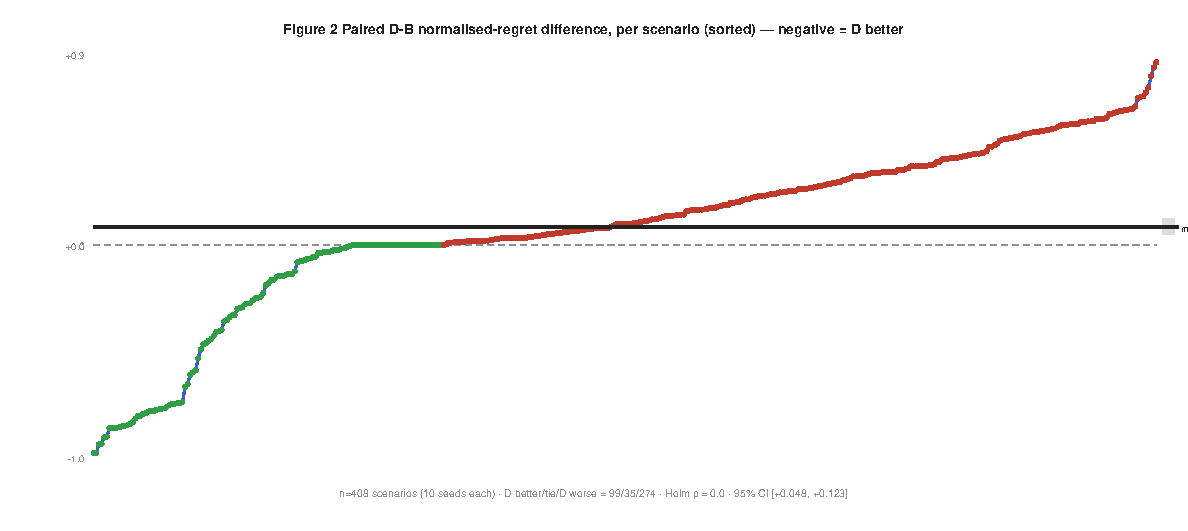
\includegraphics[width=\columnwidth]{r1_figure2}
\caption{Sorted per-scenario $\dvb$ (regret) over the 408 locked scenario means.
Bars above zero are scenarios where the full system D is worse than the
corrected decision-simulation layer B: 274 worse, 35 tied, 99 better;
mean $+0.085$, 95\% CI $[+0.048,+0.123]$.}
\label{fig:paired}
\end{figure}

%==============================================================================
\section{Results: Per-Family and Leave-One-Family-Out}\label{sec:family}
Table~\ref{tab:family} gives $\dvb$ for each of the 12 locked families;
Figure~\ref{fig:family} plots them. D is worse in \textbf{10 of 12} families and
better in \textbf{2}: \code{nonlinear\_response} ($-0.726$) and
\code{demand\_saturation} ($-0.235$). Both are \emph{censored-demand} families in
which the OLS elasticity estimate is biased toward mild values and B retains a
residual over-pricing failure (B's mean regret is $0.975$ and $0.468$ in these
two families, versus $0.013$--$0.27$ elsewhere); these are the only families
where the downstream stack's conservatism helps. The aggregate is D-worse
\emph{with and without} them: leaving out any single family gives a $\dvb$
between \textbf{$+0.050$} (drop \code{capacity\_bound}) and \textbf{$+0.159$}
(drop \code{nonlinear\_response})---every leave-one-family-out estimate is
positive (Table~\ref{tab:lofo}).

\begin{table}[!t]
\caption{Per-family $\dvb$ (mean over 34 structural scenarios $\times$ 10 seeds),
with paired scenario cluster-bootstrap 95\% CI and wins/ties/losses
(D-better / tie / D-worse).}
\label{tab:family}
\centering
\begin{tabular}{lcccc}
\toprule
Family & Mean \dvb & 95\% CI & Dir. & W/T/L \\
\midrule
\code{nonlinear\_response}  & $-0.726$ & $[-0.793,-0.651]$ & D better & $34/0/0$ \\
\code{capacity\_bound}      & $+0.477$ & $[+0.422,+0.527]$ & D worse  & $1/0/33$ \\
\code{weak\_seasonality}    & $+0.300$ & $[+0.195,+0.399]$ & D worse  & $3/0/31$ \\
\code{demand\_saturation}   & $-0.235$ & $[-0.347,-0.123]$ & D better & $23/0/11$ \\
\code{weak\_marketing}      & $+0.227$ & $[+0.133,+0.329]$ & D worse  & $1/6/27$ \\
\code{delayed\_price}       & $+0.217$ & $[+0.156,+0.285]$ & D worse  & $1/1/32$ \\
\code{asymmetric\_risk}     & $+0.189$ & $[+0.085,+0.278]$ & D worse  & $4/0/30$ \\
\code{noisy\_observations}  & $+0.164$ & $[+0.055,+0.266]$ & D worse  & $9/0/25$ \\
\code{regime\_shift}        & $+0.158$ & $[+0.085,+0.239]$ & D worse  & $9/2/23$ \\
\code{price\_elastic}       & $+0.138$ & $[+0.089,+0.195]$ & D worse  & $0/7/27$ \\
\code{strong\_seasonality}  & $+0.074$ & $[-0.030,+0.173]$ & D worse  & $14/1/19$ \\
\code{promotion\_threshold} & $+0.039$ & $[+0.017,+0.069]$ & D worse  & $0/18/16$ \\
\bottomrule
\end{tabular}
\end{table}

\begin{table}[!t]
\caption{Leave-one-family-out $\dvb$ (recomputed from raw results in the
independent recheck). Every value is positive (D worse).}
\label{tab:lofo}
\centering
\begin{tabular}{lc|lc}
\toprule
Family removed & \dvb & Family removed & \dvb \\
\midrule
\code{capacity\_bound}     & $+0.0496$ & \code{regime\_shift}      & $+0.0786$ \\
\code{weak\_seasonality}   & $+0.0657$ & \code{price\_elastic}     & $+0.0804$ \\
\code{weak\_marketing}     & $+0.0723$ & \code{strong\_seasonality}& $+0.0863$ \\
\code{delayed\_price}      & $+0.0733$ & \code{promotion\_threshold}& $+0.0894$ \\
\code{asymmetric\_risk}    & $+0.0758$ & \code{demand\_saturation} & $+0.1143$ \\
\code{noisy\_observations} & $+0.0781$ & \code{nonlinear\_response}& $+0.1590$ \\
\bottomrule
\end{tabular}
\end{table}

\begin{figure}[!t]
\centering
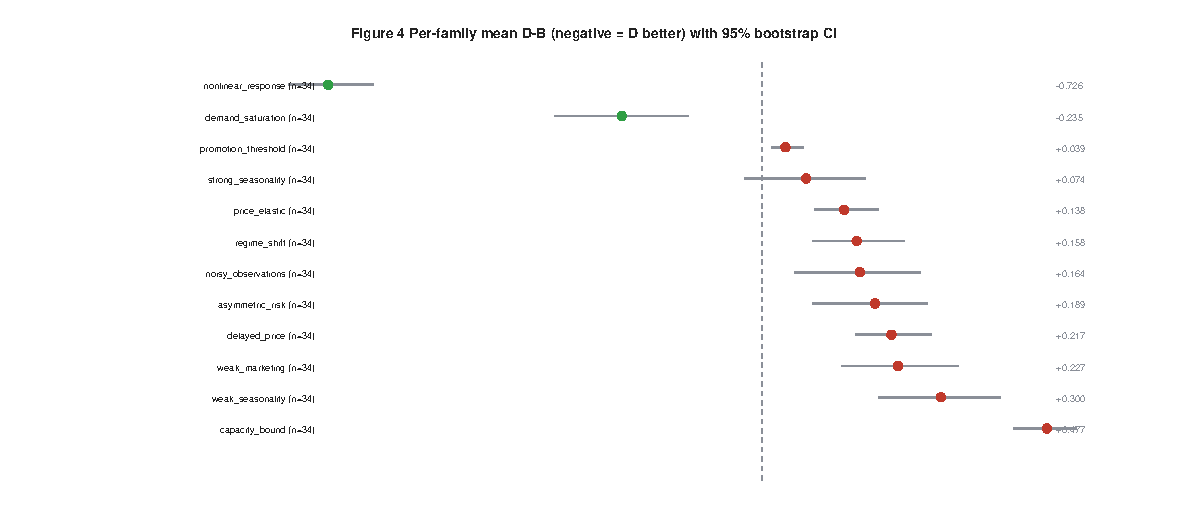
\includegraphics[width=\columnwidth]{r1_figure4}
\caption{Per-family $\dvb$ for the 12 locked families. D is worse in 10 of 12;
the two D-better families (\code{nonlinear\_response}, \code{demand\_saturation})
are censored-demand cases where B has a residual over-pricing failure.}
\label{fig:family}
\end{figure}

%==============================================================================
\section{Results: Robustness}\label{sec:robust}
Ten pre-registered perturbation types were applied at one or two severities each
to a fixed 30-scenario locked subsample (3 seeds; $1620$ perturbed runs,
0 errors): adversarial, constraint relax, constraint tighten, contradictory
signals, distribution shift, extreme-but-feasible, forecast-error bias, input
noise, missing values, and uncertainty inflation. In all \textbf{18/18} cells
the sign of $\dvb$ is unchanged from the clean subsample
(\code{primary\_conclusion\_changes} $=$ false); the perturbed $\dvb$ ranges
from $+0.046$ (heavy input noise) to $+0.339$ (adversarial). Note the clean
30-scenario subsample mean is $+0.182$---higher than the full $+0.085$ because
the subsample is weighted toward strongly D-worse families and excludes
\code{nonlinear\_response}; the robustness claim is about \emph{sign
preservation}, which the full-suite LOFO already establishes for magnitude.
Table~\ref{tab:robust} summarises.

\begin{table}[!t]
\caption{Robustness: perturbed $\dvb$ vs the 30-scenario clean subsample mean
($+0.182$). All 18 cells preserve the D-worse sign.}
\label{tab:robust}
\centering
\begin{tabular}{lcc}
\toprule
Perturbation (severities) & $\dvb$ range & Sign \\
\midrule
adversarial (1.0)                    & $+0.339$          & same \\
constraint relax (0.25, 0.5)         & $+0.210$          & same \\
constraint tighten (0.25, 0.5)       & $+0.210$          & same \\
contradictory signals (0.5, 1.0)     & $+0.167$--$+0.175$& same \\
distribution shift (0.3, 0.6)        & $+0.151$--$+0.174$& same \\
extreme but feasible (1.0)           & $+0.170$          & same \\
forecast-error bias (0.25, 0.5)      & $+0.158$--$+0.174$& same \\
input noise (0.25, 0.75)             & $+0.046$--$+0.161$& same \\
missing values (0.2, 0.4)            & $+0.179$--$+0.188$& same \\
uncertainty inflation (0.5, 1.0)     & $+0.134$--$+0.201$& same \\
\bottomrule
\end{tabular}
\end{table}

%==============================================================================
\section{Mechanism Analysis}\label{sec:mech}
This section is \textbf{associational, not causal}: the factor coefficients are
family-clustered (effective cluster count $=12$) and are not interpreted at the
individual-factor level.

\textbf{Where the loss is localised.} The mechanism analysis \emph{localises}
much of the observed degradation to the C$\to$D transition: $C\text{\_vs\_}B$ is
null while $D\text{\_vs\_}C$ is $+0.139$ (Holm $p\approx0$). The evidence
implicates the risk-gate / optimiser stage as the principal locus of the
observed performance loss; it does not establish causal attribution to any
single component. Model-free counts (Table~\ref{tab:mech}): D overrides B's
chosen action on \textbf{2336 of 4080} decisions ($57\%$); of those overrides,
\textbf{763 improve} the outcome and \textbf{1573 worsen} it (worse about
$2.1\times$ as often; Figure~\ref{fig:mech}). B's action equals the oracle
action on $62.5\%$ of decisions; D's on $34.6\%$. Per family the collapse is
sharpest exactly where B is already near-optimal:
\code{capacity\_bound} $94.1\%\!\to\!4.4\%$,
\code{asymmetric\_risk} $73.5\%\!\to\!1.2\%$,
\code{weak\_seasonality} $52.6\%\!\to\!22.6\%$ (B$\to$D optimal-action rate,
Table~\ref{tab:optaction}). D raises the optimal-action rate only in
\code{nonlinear\_response} ($0.0\%\!\to\!4.7\%$), the family where B is worst.
DecisionGPT's own internal goal-achievement metric moves the same way
($B=0.496$, $C=0.454$, $D=0.364$).

\textbf{Associational structure.} In a family-clustered OLS of $\dvb$ on
standardised scenario factors, the largest positive association is with
\code{prediction\_error} ($\beta=+0.171$, CI $[+0.136,+0.207]$) and a smaller
one with \code{risk\_exposure} ($\beta=+0.034$, CI $[+0.011,+0.052]$); i.e.\ the
D-vs-B gap is widest where the baseline forecast is least reliable and where risk
exposure is high---consistent with the downstream risk-penalty term steering the
optimiser away from B's (better) choice, but not proof of it. A separate
research diagnostic (R3, \emph{not adopted}) that rescales the risk heuristic
shifts the synthetic metric in the expected direction but is inert on the single
real price dataset available and is not promoted; the production configuration is
unchanged.

\begin{table}[!t]
\caption{Mechanism counts over 4080 locked decisions.}
\label{tab:mech}
\centering
\begin{tabular}{lc}
\toprule
Quantity & Value \\
\midrule
D overrides B's action              & $2336$ ($57.3\%$) \\
\quad of which improve outcome      & $763$ \\
\quad of which worsen outcome       & $1573$ \\
B action $=$ oracle action          & $2550$ ($62.5\%$) \\
D action $=$ oracle action          & $1410$ ($34.6\%$) \\
OLS $\dvb\sim$\code{prediction\_error} $\beta$ & $+0.171$ $[+0.136,+0.207]$ \\
OLS $\dvb\sim$\code{risk\_exposure} $\beta$    & $+0.034$ $[+0.011,+0.052]$ \\
\bottomrule
\end{tabular}
\end{table}

\begin{table}[!t]
\caption{Optimal-action rate (fraction of the 340 decisions per family whose
selected action equals the enumerated oracle action) for B and D, by locked
family. Recomputed from raw \code{results.json}.}
\label{tab:optaction}
\centering
\begin{tabular}{lcc|lcc}
\toprule
Family & B & D & Family & B & D \\
\midrule
\code{price\_elastic}      & $100.0$ & $74.1$ & \code{regime\_shift}      & $63.2$ & $45.6$ \\
\code{promotion\_threshold}& $99.4$  & $87.1$ & \code{weak\_seasonality}  & $52.6$ & $22.6$ \\
\code{capacity\_bound}     & $94.1$  & $4.4$  & \code{strong\_seasonality}& $36.2$ & $35.3$ \\
\code{delayed\_price}      & $85.3$  & $52.6$ & \code{noisy\_observations}& $34.7$ & $21.8$ \\
\code{weak\_marketing}     & $84.4$  & $54.1$ & \code{demand\_saturation} & $26.5$ & $11.2$ \\
\code{asymmetric\_risk}    & $73.5$  & $1.2$  & \code{nonlinear\_response}& $0.0$  & $4.7$  \\
\midrule
\multicolumn{6}{c}{\emph{all families:} B $62.5$, D $34.6$ (\%)} \\
\bottomrule
\end{tabular}
\end{table}

\begin{figure}[!t]
\centering
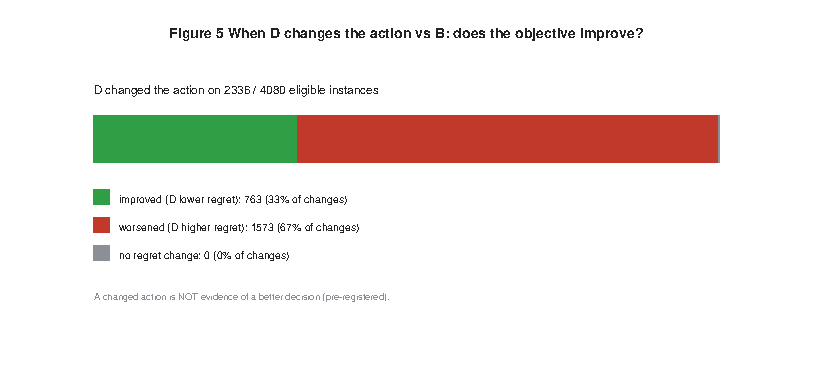
\includegraphics[width=\columnwidth]{r1_figure5}
\caption{Of the 2336 decisions where D overrides B's action, 763 improve and
1573 worsen the exogenous outcome (worse $\approx2.1\times$ as often). A changed
action is not evidence of a better decision.}
\label{fig:mech}
\end{figure}

%==============================================================================
\section{Reproducibility and Independent Recomputation}\label{sec:repro}
The frozen R1 package contains the pre-registration, the scenario manifest with
per-scenario content hashes and a suite checksum, the raw locked
\code{results.json} (SHA-256 \code{9e302f1d\ldots}), the analysis and figure
scripts, the robustness output, a 26-check machine audit
(\textbf{26/26 pass}), and per-artifact checksums. All analysis reproduces from
the frozen raw results with fixed seeds; \emph{no new locked run is required}.
An \textbf{independent recomputation} re-derived every headline statistic---the
four confirmatory contrasts, all secondary contrasts, the A/B/C/D and baseline
ladder, leave-one-family-out, the internal metric, the mechanism counts, the
12 family effects, and the 18 robustness cells---directly from
\code{results.json} with no reuse of the precomputed summaries:
\textbf{75 of 75 checks reproduce}.

%==============================================================================
\section{Contributions}\label{sec:contrib}
We claim only the following.
\begin{enumerate}
  \item A controlled, pre-registered \emph{component-level} evaluation
        methodology for integrated decision-support pipelines.
  \item An exogenous decision objective of a different functional form from the
        environment and the corrected simulator, evaluated only after action
        selection.
  \item A reproducible synthetic evaluation environment for data-constrained
        decision systems (27 families, frozen seeds and checksums).
  \item Evidence that a responsive decision-simulation layer improves on
        prediction alone in the tested environment ($B\text{\_vs\_}A$).
  \item Evidence that the tested downstream agent/risk/optimisation stack can
        \emph{degrade} decision quality relative to that layer
        ($D\text{\_vs\_}B$, robust to leave-one-family-out and 18/18
        perturbations).
  \item A mechanistic analysis localising where and under which regimes the
        degradation occurs (C$\to$D transition; optimal-action-rate collapse
        concentrated where B is near-optimal).
  \item Transparent negative-result and reproducibility reporting, including an
        independent 75/75 recomputation from the raw results.
\end{enumerate}

%==============================================================================
\section{Threats to Validity and Limitations}\label{sec:threats}
We list the limitations explicitly and do not minimise them.
\begin{enumerate}
  \item \textbf{Synthetic evaluation.} All scenarios are generated; there is no
        real transaction, market, or outcome data in the loop.
  \item \textbf{No real SME outcomes.} No real small/medium-enterprise decision
        outcomes were available at any point; the real-world validation table of
        the wider project remains not ready.
  \item \textbf{Research-only simulator correction.} R1 evaluates the
        architecture \emph{given a functioning decision-simulation layer}. The
        shipped layer is degenerate (Section~\ref{sec:diag}); the correction is
        a minimal, data-estimated elasticity model, authored by the evaluating
        team, that changes nothing else.
  \item \textbf{External validity.} The 27-family taxonomy and its parameter
        ranges are a designed artefact; ``family'' maps to ``real decision
        situation'' only by construction. Nothing here transfers to real
        businesses, ROI, customers, causal effects, deployment, or human
        decision-makers.
  \item \textbf{Baseline information advantage.} The greedy, classical-optimiser
        and oracle references have analytic access to the objective; they are
        computational benchmarks, and the paper's claims rest on the A/B/C/D
        contrasts, which do not.
  \item \textbf{Scenario-family design.} Family definitions were fixed before
        the run but were chosen by the authors; a different family set could
        shift the magnitude (the sign is robust to dropping any one family).
  \item \textbf{Finite sample.} 408 structural scenarios; the CI and
        leave-one-family-out range quantify the resulting uncertainty.
  \item \textbf{Seeds vs structural scenarios.} The 10 seeds are stochastic
        replication within a scenario, not independent structural units; every
        test uses the scenario ($n=408$) as the unit and the bootstrap resamples
        scenarios.
  \item \textbf{Elasticity-estimation error.} $\hat\varepsilon$ is an OLS
        estimate (median absolute error $0.084$ on development data; 0\% fallback
        on the locked run) and is biased mild in the two censored-demand
        families, which are exactly the families where D helps.
  \item \textbf{No real LLM.} The three agents are deterministic rule
        components; no large-language-model agent was executed, so the result
        says nothing about LLM-based multi-agent pipelines.
  \item \textbf{No human evaluation.} No human decision-maker was in the loop.
  \item \textbf{No deployment evidence.} The production configuration
        (\code{R0}/\code{D0}) is unchanged and untested here.
  \item \textbf{Mechanism-analysis limitations.} The factor OLS is
        family-clustered (12 clusters), associational, and not interpreted at the
        individual-factor level; ``localises'' and ``implicates'' are used, never
        ``causes''.
\end{enumerate}

\textbf{Response to ``this is an artifact of synthetic scenario design.''}
Four features of the design bound this concern, without claiming equivalence to
real-world validation: (i)~the scoring objective is a \emph{separate} functional
form, statically verified to import no environment or pipeline code, and applied
only after selection; (ii)~the effect holds across 12 structurally distinct
families and survives dropping any one of them (leave-one-family-out
$+0.050$ to $+0.159$); (iii)~the design, seeds, $N$ and analysis were
pre-registered and the locked test was run once; (iv)~the sign is unchanged in
all 18 pre-registered robustness perturbations. The transparent, disclosed
research-only correction and the explicit external-validity limitation above are
part of that answer, not a hedge against it.

%==============================================================================
\section{Discussion}\label{sec:disc}
In this environment, value entered the pipeline at exactly one place---the
responsive decision-simulation layer---and every component added after it either
did nothing (one agent) or removed value (the full agent-plus-optimiser stack).
The degradation is not a tail effect: D is worse than B on two thirds of
scenarios, in ten of twelve families, under leave-one-family-out, and under all
18 robustness perturbations, and the pipeline's own internal metric agrees. The
mechanism evidence---overrides that worsen outcomes $2\times$ as often as they
help, an optimal-action rate that falls from $62.5\%$ to $34.6\%$, and the gap
widening with forecast error and risk exposure---is consistent with a
risk-penalty term that over-corrects a mis-scaled risk heuristic, though we stop
short of a causal claim.

The broader reading is that a more complex pipeline does not automatically
dominate a simpler one: here a downstream stack that overrides the
simulation layer's choice on the majority of decisions moved the aggregate in
the wrong direction, and the regime-level view (Table~\ref{tab:family}) shows the
behaviour is heterogeneous---the stack helps precisely where the simpler layer
is worst (censored demand) and hurts where it is already near-optimal. This is
not a claim that simpler systems are universally better; it is a claim that the
contribution of each component must be measured, not assumed.

For practitioners assembling such stacks, the takeaway is procedural: measure
each layer against the layer below it on a held-out objective before shipping
the stack, and inspect per-regime effects rather than a single average. For this
architecture specifically, the tested deterministic multi-agent configuration
should not be assumed to add value on top of a functioning decision-simulation
layer; the production configuration is unchanged pending real-world evaluation.

%==============================================================================
\section{Conclusion}\label{sec:conc}
The controlled R1 evaluation found that making the decision-simulation layer
responsive to decision-relevant variables allowed that layer to improve upon
prediction alone ($B\text{\_vs\_}A$ mean $-0.044$, Holm $p=1\times10^{-8}$).
However, the tested downstream agent/risk/optimisation stack significantly
increased normalised regret relative to that decision-simulation baseline
($\dvb = +0.085$, 95\% CI $[+0.048,+0.123]$, Wilcoxon $p=5.4\times10^{-10}$,
Holm $p\approx0$, \rb${}=-0.469$; D worse on 274 of 408 scenarios). The
degradation was robust across leave-one-family-out analyses ($+0.050$ to
$+0.159$) and all 18 pre-registered robustness cells, and was concentrated in
action overrides introduced during the downstream transition. These findings
support component-level evaluation of integrated decision-support systems rather
than assuming that additional reasoning or optimisation layers necessarily
improve decisions.

These findings are limited to the controlled synthetic R1 environment and do not
establish real-world SME, customer, ROI, causal, deployment, or general
multi-agent-system effects. The production configuration is unchanged
(\code{R0}/\code{D0}); the research-only correction is not the shipped system;
and no large-language-model agent was evaluated. Every headline number in this
paper is independently recomputed from the frozen raw results (75/75).

%==============================================================================
\section*{Reproducibility Statement}
All R1 artifacts, the pre-registration, the analysis and figure code, the
machine audit (26/26), and the independent recomputation (75/75) are in the
project repository under \code{experiments/r1/} and \code{docs/R1\_*.md}. The
locked results file \code{results.json} has SHA-256
{\footnotesize\ttfamily 9e302f1d1cf575940e62e9abdb66393c0e7d9e9d2f2ec940abe2bd161c853065}
and the frozen experiment manifest has SHA-256
{\footnotesize\ttfamily 94aa419c703b1babb465975463b26e55255755a7687ecbecadb6db4c4c15cbff}.
No experiment was re-run for this manuscript; frozen prior artifacts
(V1, V2, R0/D0, R3, \code{experiment\_manifest.json},
\code{paper\_results\_snapshot.json}, \code{docs/PAPER\_DRAFT.md},
\code{docs/ieee\_paper/}) were verified byte-identical before and after.

%==============================================================================
\section*{Ethics and Data}
No human subjects, no personal data, and no real business data were involved.
The evaluation is entirely synthetic. No large-language-model agent was
executed. The authors declare no competing interests and no external funding for
this study.

%==============================================================================
\bibliographystyle{IEEEtran}
\bibliography{references}

\end{document}
